In diesem Kapitel soll ein Konzept erarbeitet werden, wie der Äquivalenzklassentest sinnvoll eingesetzt werden kann.
Es wird gezeigt, wie sie definiert werden können. Es wird eine Selbstüberprüfung gezeigt. 
Es werden bestehende SIL Tests überprüft, ob alle Wertebereiche abgedeckt werden.

Abbildung 6.1 soll als Beispiel einer Berechnung gelten.
% Es wird anhand von folgendem Beispiel in Abbildung 6.1 erklärt.
% Es soll die Berechnung von SDC\_AgAftTiShift getestet werden.
%Es wird als Beispiel SDC\_Current, die Berechnung für SDC\_AgAftTiShift getestet.
%Erklären, wofür diese Größe im Detail da ist.
\begin{figure}[h]
\centering
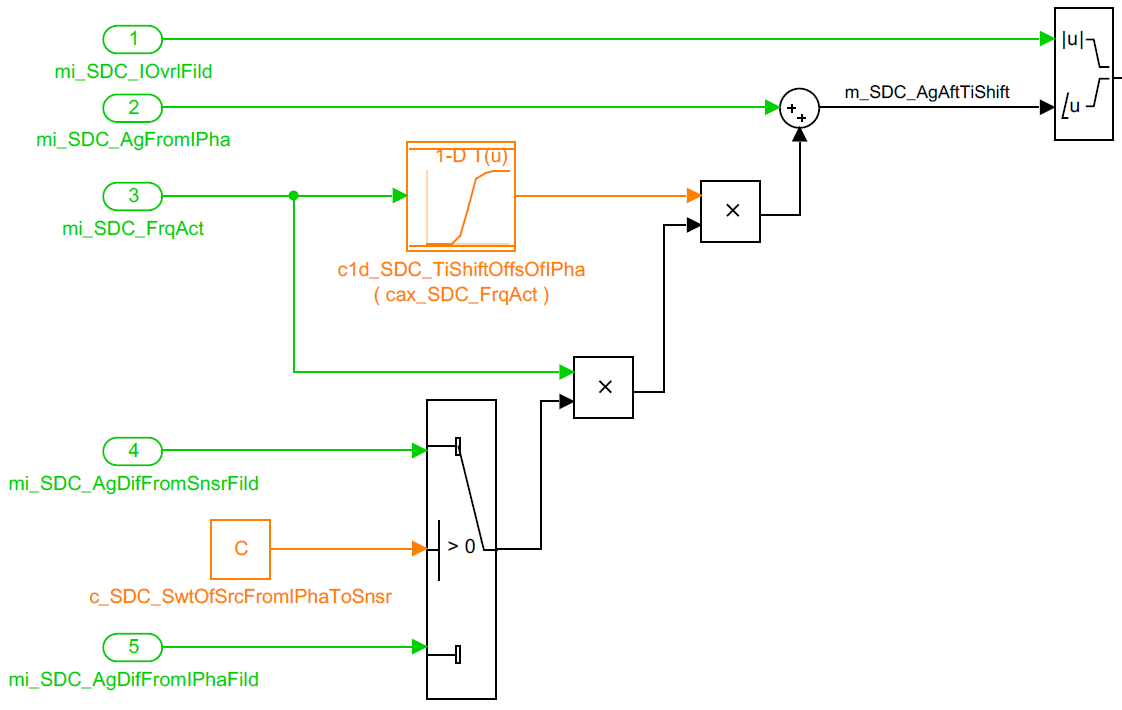
\includegraphics[scale=.9,]{Bilder/SDCDoku.png}
\caption{Beispiel einer Berechnung}
\end{figure}
Es beinhaltet eine Switch, die zwischen zwei Eingangsgrößen umschaltet. Es sind insgesamt
vier mögliche Eingangsgrößen, die durch Addition und Multiplikation sowie einer Funktion ein Ergebnis berechnen.
\section*{Definieren}
Als Grundlage dafür wird ein bestehender SIL Test genommen. Wenn der Test nach dem Requirement 
vollständig und richtig ist, so sind darin alle Werte der Signale enthalten, die für das Requirement notwendig sind.
Diese Werte können als Repräsentanten verwendet werden und dafür ein Wertebereich um den Repräsentanten
festgelegt werden. Eine Äquivalenzklasse soll ein einziges bestimmtes Verhalten abbilden. Dabei sollen alle Werte sich gleich verhalten. 
Wenn es hier Unterschiede gibt, ist es sinnvoll, sie in kleinere Wertebereiche zu zerlegen.
Beispielsweise sollen nach dem Requirement verschiedene Frequenzen getestet werden.
So werden Äquivalenzklassen
für niedrige, für mittlere, eine für hohe und eine für gefährlich hohe Werte erstellt. Es soll zweitrangig sein,
welcher Wert in der jeweiligen Klasse genommen wird, da alle Werte nach dem Requirement gleich anzusehen sind. 
\section*{Selbstüberprüfung}
Mit diesem Test soll überprüft werden, ob sie in sich Sinn machen. Es wird getestet, ob alle Äquivalenzklassen
erreichbar sind. In dem Fall des Beispiels werden alle Wertebereiche der Eingangsgrößen
der Reihe nach gesetzt und es wird überprüft, ob alle Wertebereiche des Ergebnissignals erreicht werden.
Zuerst werden alle Eingangsgrößen auf einen Repräsentanten zur Initialisierung gesetzt.
Eine Step Liste wird nach dem Minimalkriterium mit den gesetzten Äquivalenzklassen durch TPT generiert. 
Bei einer korrekten Definition sollten alle erreicht werden und die Selbstüberprüfung erfolgreich sein.
\section*{Überprüfen bestehender \ac{sil} Tests}
Es werden alle Parameter eines \ac{sil} Tests überprüft.
Dies wird mit dem \textit{Equivalence Class Coverage table} durchgeführt. Der Sinn dieses Tests ist,
den \ac{sil} Test zu validieren. Durch diesen Test wird ersichtlich, ob der \ac{sil} Test bezüglich
der Wertebereiche vollständig ist.
\section*{weitere Einsatzmöglichkeiten}
Um den Äquivalenzklassentest nutzen zu können, müssen zunächst Äquivalenzklassen definiert werden.
Das Definieren ist umfangreich und zeitaufwendig. Es bietet jedoch Vorteile, denn dadurch schafft man eine
Datenbasis an Werten als Repräsentanten beziehungsweise Wertebereichen. Nach dem Status Quo steht der Testfall
im Vordergrund und die Auswahl der Werte für den Test ist nur ein Mittel zum Zweck. Durch die neue Testart 
wird der Blickwinkel auch auf die Testwerte gelegt. Die Auswahl der Werte ist genauso wichtig wie
der Testfall selbst, denn ein Test mit den falsch gewählten Werten ist genauso hinderlich wie ein schlechtes Test Design.
Ein weiterer wichtiger Punkt ist, dass, sobald die Äquivalenzklassen definiert sind, man sie
vielfältig in allen möglichen Testfällen wiederverwenden kann. In TPT ist der Zugriff darauf beispielsweise
in der Step Liste sehr einfach
möglich durch \textit{<Signalname>->ec.random} sowie anderen Schlüsselwörtern (siehe Abschnitt 2.3).